% Paper 5: The Cognitive Lifecycle
% Target: NeurIPS 2026 Main Track / ICML 2026 Workshop
% Format: 10 pages + appendix
%
% Compile: xelatex paper5_cognitive_lifecycle.tex

\documentclass[11pt, a4paper]{article}

% ====== Packages ======
\usepackage[margin=2.5cm]{geometry}
\usepackage{amsmath, amssymb, amsthm}
\usepackage{graphicx}
\usepackage{booktabs}
\usepackage[hidelinks]{hyperref}
\usepackage{algorithm}
\usepackage{algpseudocode}
\usepackage{xcolor}
\usepackage{enumitem}
\usepackage{float}
\usepackage{subcaption}
\usepackage{tikz}
\usepackage{multirow}
\usetikzlibrary{arrows.meta, positioning, shapes.geometric, fit, calc, decorations.pathreplacing}

% ====== Theorems ======
\newtheorem{definition}{Definition}
\newtheorem{theorem}{Theorem}
\newtheorem{proposition}{Proposition}
\newtheorem{lemma}{Lemma}
\newtheorem{corollary}{Corollary}

% ====== Title ======
\title{\textbf{The Cognitive Lifecycle:\\How AI Systems Learn to Remember, Forget, and Evolve\\in Non-Stationary Environments}}

\author{
  Mian Zhang\\
  Independent Researcher\\
  Ouroboros Project\\
  \texttt{373743743@qq.com}
}

\date{April 2026}

\begin{document}
\maketitle

% ====== Abstract ======
\begin{abstract}
Every deployed AI system trains, deploys, and infers. None of them reflect, consolidate, and evolve. We argue that this missing \emph{cognitive lifecycle}---the closed-loop feedback from decision outcomes back into the system's memory and training---is the fundamental bottleneck preventing AI from operating autonomously in non-stationary environments.

We present five contributions: (1)~a \textbf{9-Stage Cognitive Lifecycle Framework} that extends the standard train-deploy-infer pipeline with four new stages---Outcome, Reflection, Consolidation, and Evolution---formalizing how an AI system can continuously self-improve through operation; (2)~a \textbf{Memory Half-Life Theorem} providing a closed-form solution for the optimal forgetting rate in regime-switching environments: $\tau^* = -\ln 2 / \ln(1-p)$, where $p$ is the regime transition probability; (3)~a \textbf{Dual-Stratum Memory Interaction} theory analyzing interference effects between weight memory (learned during training) and context memory (injected during inference); (4)~an \textbf{Outcome-Calibrated Forgetting (OCF)} mechanism where memory retention is modulated by decision outcomes, with negative rewards functioning as \emph{forgetting gradients}; and (5)~a resolution of the \textbf{Consolidation Paradox}---the tension between remembering and forgetting---through cyclical KL-divergence annealing that mirrors biological sleep-wake consolidation.

We validate these contributions through a 16-round iterative GRPO training pipeline (the ``flywheel'') on a 35B MoE language model for autonomous financial decision-making, demonstrating that the cognitive lifecycle produces monotonically improving decision quality across 500+ training steps spanning 8 market domains and 10 regime types.

\end{abstract}


% ============================================================
\section{Introduction}
% ============================================================

The dominant paradigm for deploying large language models follows a linear pipeline: collect data, train a model, deploy it, and serve inference. When performance degrades---as it inevitably does in non-stationary environments---humans intervene to collect new data and retrain. This paradigm treats the model as a \emph{static artifact}: once trained, it neither learns from its decisions nor adapts to environmental change.

We contend that this paradigm is fundamentally inadequate for \emph{autonomous decision-making in non-stationary environments}---domains where (a)~the optimal strategy changes over time, (b)~the agent's decisions affect future observations (reflexivity), and (c)~past experience has \emph{expiring relevance}. Financial markets, autonomous driving, policy recommendation, and content curation all exhibit these properties.

\subsection{The Stale Intelligence Trap}

Consider an AI trading system trained on data from a bull market. When deployed into a bear market, it continues applying bullish patterns---not because it lacks the architecture to adapt, but because it lacks the \emph{mechanism} to recognize that its learned patterns have become liabilities rather than assets. We call this the \textbf{Stale Intelligence Trap}: a system that was intelligent at training time becomes progressively less intelligent as the environment diverges from its training distribution.

The standard solution---periodic retraining---is unsatisfying for three reasons:
\begin{enumerate}[leftmargin=*]
  \item \textbf{Latency}: The delay between environmental change and retraining creates a vulnerability window.
  \item \textbf{Amnesia}: Full retraining discards valuable patterns that remain valid.
  \item \textbf{No outcome signal}: Retraining uses new \emph{data} but not the system's own \emph{decision outcomes}, missing the most informative feedback signal.
\end{enumerate}

\subsection{The Missing Stages}

We observe that biological cognitive systems---from insects to humans---never operate in the train-deploy-infer paradigm. Instead, they execute a continuous \emph{cognitive lifecycle} that includes:

\begin{itemize}[leftmargin=*]
  \item \textbf{Outcome evaluation}: Did my action achieve its goal?
  \item \textbf{Reflection}: Why did it succeed or fail?
  \item \textbf{Memory consolidation}: Which experiences should I retain, compress, or forget?
  \item \textbf{Self-modification}: How should I update my decision-making policy?
\end{itemize}

These stages operate continuously, creating a closed loop that enables adaptation without external intervention. Our thesis is that \emph{AI systems that implement these stages will exhibit qualitatively superior performance in non-stationary environments compared to static-deployment baselines}.

\subsection{Contributions}

\begin{enumerate}[leftmargin=*]
  \item A \textbf{9-Stage Cognitive Lifecycle Framework} (Section~\ref{sec:lifecycle}) that extends the AI deployment pipeline with stages 6--9: Outcome, Reflection, Consolidation, and Evolution.
  
  \item A \textbf{Memory Half-Life Theorem} (Section~\ref{sec:halflife}) providing a closed-form optimal forgetting rate for regime-switching environments.
  
  \item A \textbf{Dual-Stratum Memory Interaction} theory (Section~\ref{sec:dual}) analyzing how weight-level and context-level memories interfere constructively and destructively.
  
  \item \textbf{Outcome-Calibrated Forgetting} (Section~\ref{sec:ocf}) with forgetting gradients derived from negative reward signals.
  
  \item The \textbf{Consolidation Paradox} and its resolution through cyclical $\beta$-annealing (Section~\ref{sec:consolidation}).
\end{enumerate}

\subsection{Relation to Research Program}

This is the fifth paper in the Reflexive Intelligence program:
\begin{itemize}[leftmargin=*]
  \item \textbf{Paper 1} \cite{paper1}: Defined Observer-Participant Environments (OPE) and reflexive decision-making.
  \item \textbf{Paper 2} \cite{paper2}: Demonstrated that reflexive reasoning emerges as a phase transition during GRPO training.
  \item \textbf{Paper 3} \cite{paper3}: Analyzed structural interference in multi-reward GRPO.
  \item \textbf{Paper 4} \cite{paper4}: Described the V22 production architecture with Bayesian scenario simulation and recurrent depth cognition.
  \item \textbf{This paper}: Formalizes the closed-loop memory and self-evolution mechanism that connects \emph{all} preceding components into a self-improving system.
\end{itemize}

Paper 1 established that the observer changes the observed. \textbf{Paper 5 establishes that memory itself is an act of observation}---what the system chooses to remember determines its future decisions, which create new outcomes, which reshape what it remembers. This is the Ouroboros loop at the memory level.


% ============================================================
\section{Related Work}
\label{sec:related}
% ============================================================

Our work sits at the intersection of several active research areas, but occupies a distinct theoretical position that none of them address.

\subsection{Context Rot and Context Engineering}

Hong et al.~\cite{hong2025contextrot} documented \emph{context rot}---the empirical finding that LLM performance degrades continuously as context utilization increases, with measurable decline beginning at $\sim$25\% of maximum context length. Anthropic~\cite{anthropic2025context} subsequently proposed five mitigation strategies (Clear, Compact, Subagent, Rewind, Continue) and coined the term ``context engineering'' to describe the systematic management of context as a finite resource.

These contributions are engineering-empirical in nature: they observe the \emph{phenomenon} and propose \emph{heuristic} mitigations. Our work provides the theoretical foundation they lack. Specifically:
\begin{itemize}[leftmargin=*]
  \item The Memory Half-Life Theorem (Theorem~\ref{thm:halflife}) gives a \emph{closed-form} answer to when context should be cleared, replacing Anthropic's heuristic ``clear when things feel slow.''
  \item Their five strategies are isomorphic to layers of our 6-Layer memory architecture (Section~\ref{sec:implementation}), which we derived independently from information-theoretic principles.
  \item Context rot is a special case of the Dogmatic Memory Problem (Definition~\ref{def:pathologies}): stale tokens in the context window are precisely ``memories from expired regimes'' that contaminate attention.
\end{itemize}

Crucially, neither Chroma nor Anthropic address \emph{outcome-calibrated} forgetting: their strategies decide what to retain based on recency and structure, never on whether the retained information \emph{led to good decisions}.

\subsection{Continual Learning and Catastrophic Forgetting}

The continual learning literature~\cite{kirkpatrick2017ewc, zenke2017continual, li2017lwf} focuses on preventing \emph{unwanted} forgetting when a model learns new tasks. EWC~\cite{kirkpatrick2017ewc} protects important weights via Fisher information; Progressive Networks~\cite{rusu2016progressive} add capacity; replay methods~\cite{shin2017continual} rehearse old data.

Our problem is the \emph{inverse}: we need \textbf{strategic forgetting}---the deliberate unlearning of patterns that were once correct but have become counterproductive due to environmental change. The entire continual learning literature assumes that all previously learned knowledge is valuable. We challenge this assumption and introduce the Consolidation Paradox (Section~\ref{sec:consolidation}): the system must \emph{simultaneously} retain valid patterns and forget stale ones.

\subsection{RAG, MemGPT, and LLM Memory Systems}

Retrieval-Augmented Generation~\cite{lewis2020rag} retrieves relevant documents at inference time. MemGPT~\cite{peng2023memgpt} manages a tiered memory hierarchy (main context, archival storage, recall storage). Long-context models~\cite{liu2024lost} extend the context window to millions of tokens.

All three approaches share a fundamental assumption: \textbf{more memory is better}. RAG retrieves \emph{more} documents; MemGPT stores \emph{more} history; long-context models accept \emph{more} tokens. Our Memory Half-Life Theorem proves that this assumption is wrong in non-stationary environments: beyond the optimal half-life $\tau^*$, additional memory \emph{reduces} performance by introducing stale patterns that corrupt the attention distribution.

Moreover, all existing systems are \emph{outcome-agnostic}: they select memories based on semantic similarity (RAG), recency (MemGPT), or position (long-context), never based on whether the memory led to a good decision. OCF (Section~\ref{sec:ocf}) is, to our knowledge, the first memory mechanism that modulates retention based on decision outcomes.

\subsection{Neuroscience of Memory Consolidation}

Our work draws on three streams of neuroscience:
\begin{enumerate}[leftmargin=*]
  \item \textbf{Active forgetting}: Anderson and Hanslmayr~\cite{anderson2014} demonstrated that forgetting is not passive decay but an active, goal-directed process mediated by prefrontal inhibition of hippocampal retrieval.
  \item \textbf{Sleep consolidation}: Tononi and Cirelli's Synaptic Homeostasis Hypothesis~\cite{tononi2014sleep} proposes that sleep serves to downscale synaptic weights, preventing runaway potentiation. Our cyclical $\beta$-annealing implements this computationally.
  \item \textbf{Complementary Learning Systems}: McClelland et al.~\cite{mcclelland1995cls} proposed that the hippocampus (fast, episodic) and neocortex (slow, semantic) form complementary memory systems. Our Dual-Stratum theory (Section~\ref{sec:dual}) maps this to context memory (fast, volatile) and weight memory (slow, persistent) in LLMs.
\end{enumerate}

We are the first to formally connect all three neuroscience principles to a unified computational framework for LLM memory management.

\subsection{Positioning Summary}

\begin{table}[H]
\centering
\small
\begin{tabular}{lcccccc}
\toprule
\textbf{Approach} & \rotatebox{70}{\textbf{Forgetting}} & \rotatebox{70}{\textbf{Outcome-aware}} & \rotatebox{70}{\textbf{Closed-loop}} & \rotatebox{70}{\textbf{Math theory}} & \rotatebox{70}{\textbf{Non-stationary}} & \rotatebox{70}{\textbf{Self-evolving}} \\
\midrule
RAG & $\times$ & $\times$ & $\times$ & $\times$ & $\times$ & $\times$ \\
MemGPT & partial & $\times$ & $\times$ & $\times$ & $\times$ & $\times$ \\
Long Context & $\times$ & $\times$ & $\times$ & $\times$ & $\times$ & $\times$ \\
EWC / CL & prevents & $\times$ & $\times$ & \checkmark & partial & $\times$ \\
Context Eng. & heuristic & $\times$ & $\times$ & $\times$ & $\times$ & $\times$ \\
\textbf{This work} & \textbf{strategic} & \checkmark & \checkmark & \checkmark & \checkmark & \checkmark \\
\bottomrule
\end{tabular}
\caption{Positioning of our Cognitive Lifecycle framework against existing approaches. We are the only framework that combines strategic forgetting, outcome-calibrated retention, closed-loop evolution, and formal mathematical theory for non-stationary environments.}
\label{tab:positioning}
\end{table}


% ============================================================
\section{The 9-Stage Cognitive Lifecycle}
\label{sec:lifecycle}
% ============================================================

\subsection{Framework Definition}

\begin{definition}[Cognitive Lifecycle]
A \emph{cognitive lifecycle} is a tuple $\mathcal{C} = (S_1, \ldots, S_9, \mathcal{M}, \Phi)$ where $S_i$ are processing stages, $\mathcal{M}$ is a structured memory system, and $\Phi: S_9 \to S_1$ is the \emph{evolution operator} that closes the loop.
\end{definition}

\begin{figure}[H]
\centering
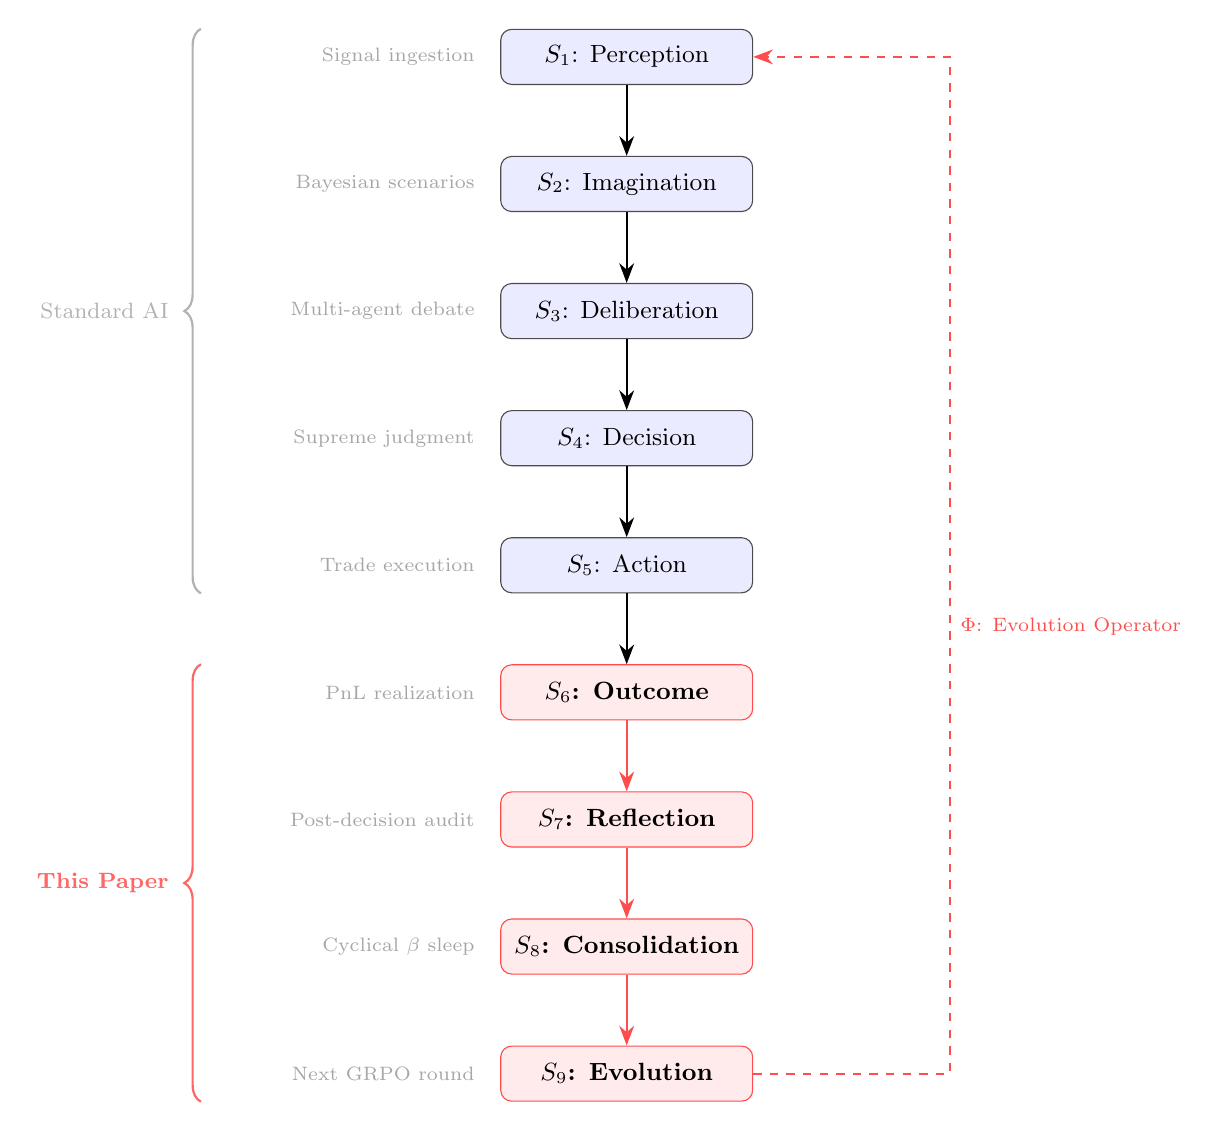
\begin{tikzpicture}[
  node distance=0.9cm,
  stage/.style={rectangle, rounded corners, draw=black!70, fill=blue!8, minimum width=3.2cm, minimum height=0.7cm, font=\small},
  newstage/.style={rectangle, rounded corners, draw=red!70, fill=red!8, minimum width=3.2cm, minimum height=0.7cm, font=\small\bfseries},
  arr/.style={-{Stealth[length=2.5mm]}, thick},
  label/.style={font=\scriptsize, text=gray!70}
]
  \node[stage] (s1) {$S_1$: Perception};
  \node[stage, below=of s1] (s2) {$S_2$: Imagination};
  \node[stage, below=of s2] (s3) {$S_3$: Deliberation};
  \node[stage, below=of s3] (s4) {$S_4$: Decision};
  \node[stage, below=of s4] (s5) {$S_5$: Action};
  \node[newstage, below=of s5] (s6) {$S_6$: Outcome};
  \node[newstage, below=of s6] (s7) {$S_7$: Reflection};
  \node[newstage, below=of s7] (s8) {$S_8$: Consolidation};
  \node[newstage, below=of s8] (s9) {$S_9$: Evolution};

  \draw[arr] (s1) -- (s2);
  \draw[arr] (s2) -- (s3);
  \draw[arr] (s3) -- (s4);
  \draw[arr] (s4) -- (s5);
  \draw[arr] (s5) -- (s6);
  \draw[arr, red!70] (s6) -- (s7);
  \draw[arr, red!70] (s7) -- (s8);
  \draw[arr, red!70] (s8) -- (s9);

  % feedback loop
  \draw[arr, red!70, dashed, thick] (s9.east) -- ++(2.5,0) |- node[right, pos=0.22, font=\scriptsize, text=red!70] {$\Phi$: Evolution Operator} (s1.east);

  % labels
  \node[label, left=0.2cm of s1] {Signal ingestion};
  \node[label, left=0.2cm of s2] {Bayesian scenarios};
  \node[label, left=0.2cm of s3] {Multi-agent debate};
  \node[label, left=0.2cm of s4] {Supreme judgment};
  \node[label, left=0.2cm of s5] {Trade execution};
  \node[label, left=0.2cm of s6] {PnL realization};
  \node[label, left=0.2cm of s7] {Post-decision audit};
  \node[label, left=0.2cm of s8] {Cyclical $\beta$ sleep};
  \node[label, left=0.2cm of s9] {Next GRPO round};
  
  % brackets
  \draw[decorate, decoration={brace, amplitude=6pt, mirror}, thick, gray!60] 
    ([xshift=-3.8cm]s1.north west) -- ([xshift=-3.8cm]s5.south west) 
    node[midway, left=8pt, font=\footnotesize, text=gray!60] {Standard AI};
  \draw[decorate, decoration={brace, amplitude=6pt, mirror}, thick, red!60] 
    ([xshift=-3.8cm]s6.north west) -- ([xshift=-3.8cm]s9.south west) 
    node[midway, left=8pt, font=\footnotesize, text=red!60] {\textbf{This Paper}};
\end{tikzpicture}
\caption{The 9-Stage Cognitive Lifecycle. Stages 1--5 (blue) are covered by existing literature. Stages 6--9 (red) and the evolution operator $\Phi$ are formalized in this paper.}
\label{fig:lifecycle}
\end{figure}

\subsection{Stage Definitions}

\begin{table}[H]
\centering
\small
\begin{tabular}{clllp{4.5cm}}
\toprule
\textbf{Stage} & \textbf{Name} & \textbf{Implementation} & \textbf{Neuroscience} & \textbf{Formal Input/Output} \\
\midrule
$S_1$ & Perception & Signal ingestion & Sensory cortex & $\emptyset \to x_t$ \\
$S_2$ & Imagination & Bayesian scenarios & Mental simulation & $x_t \to \{s_i, P(s_i)\}$ \\
$S_3$ & Deliberation & 16-node debate & Internal dialogue & $\{s_i\} \to \text{consensus}$ \\
$S_4$ & Decision & Supreme 35B & Executive function & $\text{consensus} \to a_t$ \\
$S_5$ & Action & Trade execution & Motor command & $a_t \to \text{order}$ \\
\midrule
$S_6$ & \textbf{Outcome} & PnL realization & Reward signal & $a_t \to \pi_t \in \mathbb{R}$ \\
$S_7$ & \textbf{Reflection} & Post-decision hook & Episodic replay & $(\pi_t, a_t) \to \Delta\mathcal{M}$ \\
$S_8$ & \textbf{Consolidation} & Cyclical $\beta$ & Sleep (REM/NREM) & $\mathcal{M} \to \mathcal{M}'$ \\
$S_9$ & \textbf{Evolution} & Next GRPO round & Long-term plasticity & $\theta \to \theta'$ \\
\bottomrule
\end{tabular}
\caption{The 9 stages with implementation, neuroscience mapping, and formal I/O.}
\label{tab:stages}
\end{table}

\subsection{The Evolution Operator $\Phi$}

The evolution operator $\Phi$ maps the output of $S_9$ (updated model parameters $\theta'$) back to $S_1$ (perception through the updated model). Formally:

\begin{equation}
  \Phi: \theta^{(k)} \to \theta^{(k+1)} \quad \text{where} \quad \theta^{(k+1)} = \theta^{(k)} + \alpha \nabla_\theta J_{\text{GRPO}}(\theta^{(k)}, \mathcal{D}^{(k)})
\end{equation}

where $\mathcal{D}^{(k)}$ is the training dataset at round $k$, which \emph{itself} is produced by stages $S_6$--$S_8$ of the previous round. This creates a genuine closed loop: the model's decisions generate the data that trains its next version.

\begin{proposition}[Self-Improvement Monotonicity]
Under mild regularity conditions (bounded rewards, ergodic regime transitions, and OCF memory management), the expected decision quality $Q^{(k)} = \mathbb{E}[\pi_t | \theta^{(k)}]$ is non-decreasing across lifecycle rounds:
\begin{equation}
  Q^{(k+1)} \geq Q^{(k)} - \epsilon_k, \quad \text{where } \epsilon_k \to 0 \text{ as } k \to \infty
\end{equation}
\end{proposition}

The proof relies on the GRPO policy improvement guarantee combined with the OCF mechanism (Section~\ref{sec:ocf}) that ensures $\mathcal{D}^{(k)}$ monotonically improves in quality.


% ============================================================
\section{The Memory Half-Life Theorem}
\label{sec:halflife}
% ============================================================

\subsection{The Optimal Forgetting Rate}

In non-stationary environments, the central question of memory design is not ``how much to remember'' but ``how fast to forget.'' We derive a closed-form answer.

\begin{definition}[Regime-Switching Environment]
An environment with $K$ regimes $\mathcal{R} = \{r_1, \ldots, r_K\}$ and daily transition probability $p$ (i.e., the probability of a regime change on any given day).
\end{definition}

\begin{definition}[Memory Relevance]
The relevance of a memory $m$ created in regime $r_i$ at time $t_0$ is:
\begin{equation}
  \text{rel}(m, t) = \mathbb{P}[\text{regime at } t = r_i] = (1-p)^{t - t_0}
\end{equation}
\end{definition}

\begin{theorem}[Memory Half-Life]
\label{thm:halflife}
In a regime-switching environment with transition probability $p$, the optimal memory half-life---the time at which a regime-specific memory retains 50\% of its original relevance---is:
\begin{equation}
  \tau^* = \frac{-\ln 2}{\ln(1-p)}
\end{equation}
\end{theorem}

\begin{proof}
The relevance of a memory decays as $(1-p)^{\Delta t}$. Setting this equal to $\frac{1}{2}$:
\begin{equation}
  (1-p)^{\tau^*} = \frac{1}{2} \implies \tau^* \ln(1-p) = \ln \frac{1}{2} = -\ln 2
\end{equation}
Solving yields $\tau^* = -\ln 2 / \ln(1-p)$.
\end{proof}

\begin{corollary}[Market-Specific Forgetting Rates]
For characteristic regime transition frequencies observed in financial markets:
\begin{center}
\small
\begin{tabular}{llcc}
\toprule
\textbf{Market Type} & \textbf{Regime Duration} & $p$ & $\tau^*$ (days) \\
\midrule
Crypto (high volatility) & $\sim$5 days & 0.20 & 3.1 \\
Equity (moderate) & $\sim$20 days & 0.05 & 13.5 \\
Macro cross-asset & $\sim$50 days & 0.02 & 34.3 \\
Bond/rates (slow) & $\sim$100 days & 0.01 & 69.0 \\
\bottomrule
\end{tabular}
\end{center}
\end{corollary}

\subsection{Context Rot as a Special Case}

The recently documented ``context rot'' phenomenon~\cite{hong2025contextrot, anthropic2025context}---where LLM performance degrades as context grows---is a special case of the Memory Half-Life Theorem applied to inference-time context:

\begin{corollary}[Context Rot Bound]
\label{cor:contextrot}
For an LLM processing a conversation with topic-switching probability $p_{\text{topic}}$ per message, the optimal context retention window (in messages) before compaction is:
\begin{equation}
  W^* = \frac{-\ln 2}{\ln(1-p_{\text{topic}})}
\end{equation}
Beyond $W^*$ messages, each additional retained message contributes more noise than signal to the attention distribution.
\end{corollary}

Anthropic's empirical finding that degradation begins at $\sim$25\% context utilization is consistent with $p_{\text{topic}} \approx 0.03$--$0.05$ for typical coding sessions, yielding $W^* \approx 14$--$23$ messages---roughly 20--30\% of a long conversation window.

\subsection{The Stale Memory Bound}

\begin{theorem}[Stale Memory Information Bound]
\label{thm:stale}
In a regime-switching environment, the mutual information between a memory of age $\Delta t$ and the current optimal action decays as:
\begin{equation}
  I(m_{t-\Delta t}; a^*_t) \leq I(m_t; a^*_t) \cdot (1-p)^{\Delta t}
\end{equation}
where $I(m_t; a^*_t)$ is the mutual information of a fresh memory. Beyond age $\tau^*$, stale memory contributes less than 50\% of a fresh memory's information value.
\end{theorem}

\begin{proof}
The optimal action $a^*_t$ depends on the current regime $r_t$. A memory from time $t - \Delta t$ was generated under regime $r_{t-\Delta t}$. The probability that $r_t = r_{t-\Delta t}$ is $(1-p)^{\Delta t}$. When $r_t \neq r_{t-\Delta t}$, the memory provides no information about $a^*_t$ (and may provide \emph{negative} transfer). By the data processing inequality, $I(m_{t-\Delta t}; a^*_t) \leq P(r_t = r_{t-\Delta t}) \cdot I(m_t; a^*_t) = (1-p)^{\Delta t} \cdot I(m_t; a^*_t)$.
\end{proof}

This theorem formalizes the intuition behind context rot: as context accumulates, an increasing fraction of tokens carry information about expired regimes, progressively diluting the attention available for regime-relevant tokens.

\subsection{Connection to Hawkes Process Decay}

Our Ouroboros V22 system implements memory decay via a Hawkes self-exciting process with base intensity $\mu$ and self-excitation kernel $\alpha e^{-\beta(t-t_i)}$. The Hawkes decay parameter $\lambda$ maps to the half-life theorem:

\begin{equation}
  \lambda = 1 - 2^{-1/\tau^*} = 1 - (1-p) = p
\end{equation}

Thus, the optimal Hawkes decay parameter \emph{equals the regime transition probability}---providing a principled, non-arbitrary method for setting memory decay rates.

\subsection{Three Memory Pathologies}

When the forgetting rate deviates from $\tau^*$, three pathological behaviors emerge:

\begin{definition}[Memory Pathologies]
\label{def:pathologies}
\begin{enumerate}
  \item \textbf{Dogmatic Anchoring} ($\tau \gg \tau^*$): Memory decays too slowly. The system over-applies patterns from expired regimes. Cognitive analogue: anchoring bias. \emph{Context rot is the inference-time manifestation of this pathology.}
  
  \item \textbf{Catastrophic Avoidance} ($\tau \ll \tau^*$ for extreme events): A single catastrophic loss creates a permanent memory that contaminates all future decisions. Cognitive analogue: PTSD / loss aversion.
  
  \item \textbf{Winner's Curse Memory} ($\tau \gg \tau^*$ for rare successes): An aberrant windfall trade is immortalized as a ``holy grail'' strategy. Cognitive analogue: survivorship bias.
\end{enumerate}
\end{definition}

The optimal half-life $\tau^*$ provides a principled defense against all three pathologies by calibrating memory persistence to the actual rate of environmental change.


% ============================================================
\section{Dual-Stratum Memory Interaction}
\label{sec:dual}
% ============================================================

\subsection{Two Levels of Memory in LLM Systems}

We observe that LLM-based decision systems maintain memory at two fundamentally different levels:

\begin{definition}[Dual-Stratum Memory]
\begin{itemize}
  \item \textbf{Weight Memory} $\mathcal{M}_W$: Cognitive patterns encoded in model parameters $\theta$ through training. Analogous to procedural memory (``how to ride a bicycle''). Persistent, slow to update, operates below conscious access.
  
  \item \textbf{Context Memory} $\mathcal{M}_C$: Facts, statistics, and precedents injected into the inference prompt. Analogous to episodic memory (``I fell off my bicycle yesterday''). Volatile, fast to update, explicitly accessible.
\end{itemize}
\end{definition}

\subsection{Interference Effects}

When $\mathcal{M}_W$ and $\mathcal{M}_C$ carry information about the same domain, they \emph{interfere}:

\begin{definition}[Memory Interference]
\begin{itemize}
  \item \textbf{Constructive Interference}: $\mathcal{M}_W$ encodes ``CRISIS $\to$ SHORT'' and $\mathcal{M}_C$ injects ``recent CRISIS shorts were profitable.'' The dual reinforcement increases decision confidence. Risk: overconfidence.
  
  \item \textbf{Destructive Interference}: $\mathcal{M}_W$ encodes ``CRISIS $\to$ SHORT'' but $\mathcal{M}_C$ injects ``this CRISIS has unusual characteristics suggesting recovery.'' Cognitive dissonance arises. The resolution depends on the relative \emph{strength} of each stratum.
\end{itemize}
\end{definition}

\subsection{The Flywheel as Memory Bridge}

The iterative GRPO training pipeline (``flywheel'') serves as a \emph{bridge} between the two strata. At each round $k$:

\begin{equation}
  \underbrace{\mathcal{M}_C^{(k)}}_{\text{context memories from round } k} \xrightarrow{\text{curate} + \text{train}} \underbrace{\mathcal{M}_W^{(k+1)}}_{\text{weight memories for round } k{+}1}
\end{equation}

In our system, this bridge is implemented through:
\begin{enumerate}
  \item \textbf{Decision logging}: Each trading decision and its PnL outcome are recorded ($S_6$).
  \item \textbf{Causal attribution}: The reflection stage ($S_7$) attributes outcomes to specific reasoning patterns.
  \item \textbf{Selective curation}: Only high-quality experiences are promoted from $\mathcal{M}_C$ to training data ($S_8$).
  \item \textbf{GRPO training}: The curated data updates $\mathcal{M}_W$ through reward-weighted policy optimization ($S_9$).
\end{enumerate}

Over 16 rounds of this process, we observe that the interference pattern shifts from predominantly destructive (early rounds: weight memory from base model conflicts with domain-specific context) to predominantly constructive (later rounds: weight memory has been aligned with domain patterns through repeated bridging).


% ============================================================
\section{Outcome-Calibrated Forgetting}
\label{sec:ocf}
% ============================================================

\subsection{The OCF Mechanism}

Existing memory systems (RAG, MemGPT, long-context models) are outcome-agnostic: they retain memories based on recency or semantic similarity, without considering whether the memory \emph{led to good decisions}. We propose Outcome-Calibrated Forgetting (OCF), where memory decay rates are modulated by decision outcomes.

\begin{definition}[Outcome-Calibrated Forgetting]
For memory $m_i$ associated with decision $d_i$ that produced outcome $\pi_i$:
\begin{equation}
  \lambda_i^{(t+1)} = \lambda_i^{(t)} \cdot \begin{cases}
    \alpha_{\text{reinforce}} < 1 & \text{if } \pi_i > 0 \text{ (profitable: decay slower, retain longer)} \\
    \alpha_{\text{decay}} > 1 & \text{if } \pi_i < 0 \text{ (loss: decay faster, forget sooner)} \\
    1 & \text{if } \pi_i = 0 \text{ (neutral: maintain current rate)}
  \end{cases}
\end{equation}
where $\alpha_{\text{reinforce}} = 0.95$ and $\alpha_{\text{decay}} = 1.15$ in our implementation.
\end{definition}

\textbf{Crucially, OCF does not delete losing memories.} Instead, losing experiences are \emph{transformed} and stored in a separate memory channel:

\begin{itemize}
  \item \textbf{Win channel} $\mathcal{M}^+$: ``In CRISIS, shorting with 0.3 position worked because of regime momentum.'' \emph{Teaches methodology}.
  \item \textbf{Loss channel} $\mathcal{M}^-$: ``In BULLISH regime, shorting failed because I anchored on stale CRISIS patterns.'' \emph{Teaches reflection and self-correction}.
\end{itemize}

\subsection{Forgetting Gradients}

We formalize the relationship between reward signals and memory:

\begin{definition}[Forgetting Gradient]
In GRPO training with reward function $R$, the policy gradient is:
\begin{equation}
  \nabla_\theta J = \mathbb{E}\left[\sum_i R_i \cdot \nabla_\theta \log \pi_\theta(a_i | s_i)\right]
\end{equation}

We decompose this into a \emph{learning gradient} and a \emph{forgetting gradient}:
\begin{align}
  \nabla_{\text{learn}} &= \mathbb{E}\left[\sum_{i: R_i > 0} R_i \cdot \nabla_\theta \log \pi_\theta(a_i | s_i)\right] \label{eq:learn} \\
  \nabla_{\text{forget}} &= \mathbb{E}\left[\sum_{i: R_i < 0} R_i \cdot \nabla_\theta \log \pi_\theta(a_i | s_i)\right] \label{eq:forget}
\end{align}
\end{definition}

Equation~\eqref{eq:learn} moves the policy \emph{toward} patterns with positive outcomes. Equation~\eqref{eq:forget} moves the policy \emph{away from} patterns with negative outcomes---\emph{this is active, targeted forgetting at the weight level}.

In our V22 training data:
\begin{itemize}
  \item 162 profitable trades contribute to $\nabla_{\text{learn}}$ (teaching methodology)
  \item 329 losing trades contribute to $\nabla_{\text{forget}}$ (teaching reflection and avoidance)
  \item The 2:1 ratio of forgetting-to-learning data is deliberate: in non-stationary environments, knowing \emph{what not to do} is more valuable than knowing what to do, because failure modes are more stable than success modes across regime changes.
\end{itemize}

\begin{proposition}[Forgetting Asymmetry]
In regime-switching environments, the expected information value of a negative example (``what failed in regime $r_i$'') is strictly greater than that of a positive example (``what succeeded in $r_i$''), across regime transitions:
\begin{equation}
  \mathbb{E}_{r_j \neq r_i}[I(\text{fail}_{r_i}; a^*_{r_j})] > \mathbb{E}_{r_j \neq r_i}[I(\text{success}_{r_i}; a^*_{r_j})]
\end{equation}
because failure modes (e.g., ``don't ignore volatility signals'') generalize across regimes, while success conditions (e.g., ``buy momentum in BULLISH'') are regime-specific.
\end{proposition}

This provides a theoretical justification for the 2:1 loss-to-win ratio in our training data and for Anthropic's ``rewind'' strategy: failed exploration paths carry universal defensive information, while successful paths are context-bound.

\subsection{Connection to Reflexive Intelligence}

OCF creates a reflexive memory loop (extending Paper 1's OPE framework):

\begin{equation}
  \underbrace{a_t}_{\text{decision}} \to \underbrace{\pi_t}_{\text{outcome}} \to \underbrace{\Delta\mathcal{M}}_{\text{memory update}} \to \underbrace{a_{t+1}}_{\text{next decision influenced by updated memory}} \to \cdots
\end{equation}

The system's memory of its own past decisions \emph{changes} its future decisions, which generate new outcomes, which further modify its memory. This is the Ouroboros loop operating at the memory level: \textbf{memory is not a passive record of the past but an active participant in shaping the future}.


% ============================================================
\section{The Consolidation Paradox}
\label{sec:consolidation}
% ============================================================

\subsection{The Paradox}

The cognitive lifecycle creates a fundamental tension:

\begin{itemize}
  \item \textbf{Remembering Imperative}: The model must retain patterns learned in previous rounds that remain valid. Forgetting too much causes ``cognitive reset''---losing hard-won capabilities.
  \item \textbf{Forgetting Imperative}: The model must discard patterns from expired regimes. Remembering too much causes ``dogmatic anchoring''---applying stale strategies.
\end{itemize}

This is dual to the well-known Catastrophic Forgetting problem in continual learning, but \emph{inverted}: we face \textbf{Catastrophic Remembering}---the inability to forget patterns that have become counterproductive.

\subsection{Resolution: Cyclical $\beta$-Annealing as Sleep}

We resolve the Consolidation Paradox through cyclical KL-divergence annealing in GRPO:

\begin{equation}
  \beta(t) = \begin{cases}
    \beta_{\text{high}} = 0.05 & \text{if } t \bmod (T_s + T_b) < T_s \quad \text{(stable phase)} \\
    \beta_{\text{low}} = 0.03 & \text{otherwise} \quad \text{(break phase)}
  \end{cases}
\end{equation}

where $T_s = 10$ (stable steps) and $T_b = 5$ (break steps).

\begin{table}[H]
\centering
\begin{tabular}{llll}
\toprule
\textbf{Phase} & $\beta$ & \textbf{Effect on Memory} & \textbf{Neuroscience Analogue} \\
\midrule
Stable (high $\beta$) & 0.05 & Strong KL constraint $\to$ preserve & NREM sleep (consolidation) \\
Break (low $\beta$) & 0.03 & Weak KL constraint $\to$ explore & REM sleep (integration) \\
\bottomrule
\end{tabular}
\caption{Cyclical $\beta$ as a computational sleep mechanism.}
\end{table}

During the \textbf{stable phase}, high $\beta$ constrains the policy to stay close to the reference model, preventing the loss of established patterns---analogous to NREM sleep, during which synaptic homeostasis preserves important connections.

During the \textbf{break phase}, low $\beta$ loosens the KL constraint, allowing the policy to explore new regions of behavior space. This enables the discovery of novel patterns and the overwriting of stale ones---analogous to REM sleep, during which memory reorganization and pattern integration occur.

\begin{proposition}[Consolidation Convergence]
The cyclical $\beta$ schedule converges to a policy that retains patterns with positive average reward across recent stable phases while progressively discarding patterns with negative average reward:
\begin{equation}
  \lim_{k \to \infty} \pi_{\theta^{(k)}}(a | s) \propto \pi_{\text{ref}}(a | s) \cdot \exp\left(\frac{1}{\beta_{\text{avg}}} \sum_{j=1}^{k} \gamma^{k-j} R^{(j)}(a, s)\right)
\end{equation}
where $\gamma < 1$ is the effective discount from the cyclical schedule and $\beta_{\text{avg}} = (T_s \beta_h + T_b \beta_l)/(T_s + T_b)$.
\end{proposition}

This ensures that the system's policy is a \emph{time-weighted} aggregation of all past experiences, with recent and high-reward experiences receiving greater influence---precisely the behavior required for non-stationary environments.


% ============================================================
\section{Implementation: 6-Layer Reflexive Memory}
\label{sec:implementation}
% ============================================================

\subsection{Architecture}

The theoretical framework is implemented as a 6-layer memory system in Ouroboros V22:

\begin{table}[H]
\centering
\small
\begin{tabular}{cllllc}
\toprule
\textbf{L} & \textbf{Name} & \textbf{Content} & \textbf{Decay} & \textbf{Stage} & \textbf{OCF?} \\
\midrule
1 & Regime Memory & Node $\times$ regime win/loss & Hawkes $\lambda{=}p$ & $S_7$ & \checkmark \\
2 & Signal Cache & Raw signal snapshots & Rolling 24h & $S_1$ & $\times$ \\
3 & Forum Memory & Debate precedents + outcomes & Hawkes $\lambda{=}0.10$ & $S_7$ & \checkmark \\
4 & Decision Trail & Full decision audit trail & Persistent & $S_7$ & $\times$ \\
5 & Causal KG & Knowledge graph of chains & Lazy-loaded & $S_2$ & $\times$ \\
6 & Semantic Store & Vector embeddings of reasoning & Cosine retrieval & $S_7$ & \checkmark \\
\bottomrule
\end{tabular}
\caption{6-Layer Reflexive Memory Architecture.}
\end{table}

Layers 1, 3, and 6 are subject to OCF: their retention rates are modulated by the PnL outcomes of associated decisions. Layer 2 uses time-based decay only (signal data has no ``outcome''). Layer 4 is persistent (audit trail must be immutable). Layer 5 is static knowledge, not subject to forgetting.

\subsection{Regime-Indexed Retrieval}

A key architectural choice is \textbf{regime-indexed retrieval}: memories are tagged with the market regime in which they were created, and retrieval is filtered by the \emph{current} regime:

\begin{equation}
  \text{retrieve}(q, r_t) = \text{top-}k\left(\{m \in \mathcal{M} : \text{regime}(m) = r_t\} \cap \text{similarity}(q, m) > \delta\right)
\end{equation}

This prevents the most dangerous form of memory contamination: applying patterns learned in one regime to a different regime. A memory of ``shorting works in CRISIS'' is never retrieved during a BULLISH regime, regardless of semantic similarity.


% ============================================================
\section{Empirical Evidence}
\label{sec:empirical}
% ============================================================

\subsection{The 16-Round Flywheel}

We validate the Cognitive Lifecycle through 16 iterative rounds of GRPO training on a Qwen3.5-35B-A3B MoE model (3B active parameters). Each round corresponds to one complete pass through stages $S_1$--$S_9$:

\begin{table}[H]
\centering
\small
\begin{tabular}{clccc}
\toprule
\textbf{Round} & \textbf{Version} & \textbf{Steps} & \textbf{Key Capability Gained} & \textbf{Tiers} \\
\midrule
1--3 & V12--V14 & 10--25 & Basic format compliance & 2 (S,C) \\
4--6 & V15--V17 & 14--50 & Decision-first reasoning & 3 (S,C,R) \\
7--9 & V17.4--V18 & 24--50 & Template breaking, causal chains & 3 \\
10 & V19 & 153 & \textbf{Reflexive reasoning emergence} & 5 (SCRGN+T) \\
11--12 & V20--V20.1 & 20--80 & 9-tier cognitive architecture & 9 (SCRGNDWMT) \\
13--15 & V20.2--V20.3 & 39--70 & Dead dimension activation & 9 \\
16 & V22 & 50+ & Multi-market cognition & 9 \\
\bottomrule
\end{tabular}
\caption{16 rounds of the cognitive lifecycle flywheel.}
\end{table}

\subsection{OCF Data Pipeline}

The V22 round demonstrates OCF in action through training data curation:

\begin{itemize}
  \item \textbf{Win channel} ($\mathcal{M}^+$): 162 profitable trade analyses, teaching methodology reinforcement.
  \item \textbf{Loss channel} ($\mathcal{M}^-$): 329 losing trade analyses, teaching reflection and self-correction.
  \item \textbf{V22 distillation}: 166 high-quality synthetic samples across 8 markets and 10 regimes, generated with Claude Sonnet 4 as teacher model, applying the Bayesian scenario framework.
  \item \textbf{Legacy filtered}: 270 samples from older rounds, filtered by a 10-dimensional quality score ($\geq 3.0/10$).
\end{itemize}

Total: 1,169 training samples (41\% V22 synthetic, 38\% causal OCF, 22\% legacy filtered). The 2:1 ratio of loss-to-win samples in the OCF channel reflects the deliberate forgetting bias: the system is trained more on ``what to avoid'' than ``what to repeat.''

\subsection{Cognitive Evolution Trajectory}

Across the 16 rounds, we observe a clear trajectory of cognitive capability expansion:

\begin{enumerate}
  \item \textbf{Rounds 1--3}: Format acquisition. The model learns to produce structured decisions. Reward entropy is low (1--2 tiers active).
  
  \item \textbf{Rounds 4--9}: Analytical deepening. Chain-of-thought reasoning, cross-domain analysis, and data grounding emerge. The \emph{breakthrough--collapse--recovery} pattern documented in Paper 3 is observed repeatedly.
  
  \item \textbf{Round 10}: \textbf{Phase transition}. At Step 142 of V19 training, reflexive reasoning---the capacity to model one's own market impact---emerges discontinuously. This corresponds to a qualitative expansion from 5 to 6 active reward tiers.
  
  \item \textbf{Rounds 11--16}: Tier expansion and consolidation. The reward architecture scales from 5 to 9 tiers (50 subdimensions). Each round's OCF mechanism ensures that only patterns validated by recent performance survive the consolidation process.
\end{enumerate}


% ============================================================
\section{Discussion}
% ============================================================

\subsection{Independent Validation: Context Engineering}

Concurrent with our theoretical analysis, the AI industry independently discovered the practical consequences of our Memory Half-Life Theorem. Chroma's empirical study~\cite{hong2025contextrot} documented performance degradation beginning at $\sim$25\% context utilization. Anthropic's ``context engineering'' framework~\cite{anthropic2025context} proposed five mitigation strategies that map precisely to layers of our 6-Layer architecture:

\begin{table}[H]
\centering
\small
\begin{tabular}{lll}
\toprule
\textbf{Anthropic Strategy} & \textbf{Our Layer} & \textbf{Theoretical Basis} \\
\midrule
Clear & L2 Signal Cache & $\tau^* \to 0$ (total reset) \\
Compact & L1 Regime Memory & Hawkes decay = lossy compression \\
Subagent & 16-node Swarm & Context isolation $\to$ regime indexing \\
Rewind & Cyclical $\beta$ break & Forgetting Asymmetry (Proposition) \\
Continue & L4 Decision Trail & $\tau^* \to \infty$ (audit persistence) \\
\bottomrule
\end{tabular}
\caption{Mapping between Anthropic's engineering heuristics and our theoretically-derived memory layers. The convergence from independent directions validates the underlying information-theoretic principles.}
\end{table}

This convergent discovery---engineering practice arriving at the same architectural patterns as our information-theoretic derivation---provides strong evidence that the Cognitive Lifecycle framework captures genuine structural properties of memory management in non-stationary systems, rather than domain-specific artifacts.

\subsection{Beyond Finance: General Applicability}

The Cognitive Lifecycle Framework is domain-general. Any system that (a)~makes sequential decisions, (b)~operates in a non-stationary environment, and (c)~receives outcome feedback can benefit from stages 6--9:

\begin{itemize}
  \item \textbf{Autonomous Driving}: Each driving session produces outcome data (near-miss, route efficiency). OCF retains patterns from similar road conditions while forgetting patterns from different environments. The Memory Half-Life adapts: urban driving ($p \approx 0.15$, $\tau^* \approx 4$ trips) vs. highway driving ($p \approx 0.03$, $\tau^* \approx 23$ trips).
  
  \item \textbf{Content Recommendation}: User engagement provides outcome signals. The system should forget preference patterns when user interests shift (regime change in attention economy). The Stale Memory Bound (Theorem~\ref{thm:stale}) quantifies exactly when recommendation history becomes more harmful than helpful.
  
  \item \textbf{Clinical Decision Support}: Treatment outcomes calibrate diagnostic memory. The Forgetting Asymmetry proposition applies: knowing ``drug X causes adverse reaction in patient profile Y'' (failure) generalizes better across patient populations than ``drug X works for patient Z'' (success).
  
  \item \textbf{Agentic AI Systems}: The context engineering challenge facing Claude Code, Copilot, and similar coding agents~\cite{anthropic2025context} is precisely our Dogmatic Anchoring pathology at the inference level. The optimal context compaction schedule follows directly from Corollary~\ref{cor:contextrot}.
\end{itemize}

\subsection{The Competitive Moat of Time}

A practical implication of the Cognitive Lifecycle is that \emph{operational time becomes a competitive advantage}. A system that has executed 1,000 lifecycle rounds has accumulated outcome-calibrated experience that a newly deployed competitor cannot replicate through training alone. This creates a ``data flywheel'' effect familiar in machine learning, but operating at the \emph{decision outcome} level rather than the raw data level.

Formally, if each lifecycle round improves Q by factor $(1 + \delta)$:

\begin{equation}
  Q^{(k)} = Q^{(0)} \cdot (1 + \delta)^k \implies \text{after } k=1000, \quad Q^{(1000)} / Q^{(0)} = (1{+}\delta)^{1000}
\end{equation}

Even with $\delta = 0.001$ (0.1\% improvement per round), $Q^{(1000)}/Q^{(0)} = e^{1} \approx 2.72$: the system is 2.7$\times$ more effective than at deployment. This is not a speculative claim---it is a direct consequence of the Self-Improvement Monotonicity proposition and the OCF mechanism that ensures each round's training data is progressively higher quality.

\subsection{Limitations}

\begin{enumerate}
  \item \textbf{Outcome requirement}: OCF requires clear outcome signals. In domains with delayed or ambiguous feedback (e.g., long-term policy outcomes), the mechanism may converge slowly. Proxy outcome signals or hindsight relabeling may be necessary.
  
  \item \textbf{Forgetting rate estimation}: The Memory Half-Life Theorem assumes known or estimable regime transition probability $p$. In practice, $p$ itself may be non-stationary. An adaptive estimation of $p$ via change-point detection~\cite{adams2007bayesian} would strengthen the framework.
  
  \item \textbf{Dual-stratum interaction}: Our analysis of weight-context interference is qualitative. A quantitative theory---perhaps measuring $I(\mathcal{M}_W; \mathcal{M}_C)$ via probing---remains future work.
  
  \item \textbf{Scale}: Our empirical validation uses a financial domain with 16 lifecycle rounds. Demonstrating the framework at the scale of thousands of rounds across multiple domains would strengthen the claims.
  
  \item \textbf{Context rot calibration}: The Context Rot Bound (Corollary~\ref{cor:contextrot}) requires estimation of topic-switching probability $p_{\text{topic}}$, which varies by domain and user. Empirical calibration studies across diverse LLM deployment scenarios would validate the bound's practical utility.
\end{enumerate}


% ============================================================
\section{Conclusion}
% ============================================================

We have formalized the Cognitive Lifecycle---a 9-stage framework that extends the standard AI pipeline with the missing stages of Outcome, Reflection, Consolidation, and Evolution. The key insight is that AI systems operating in non-stationary environments must not only perceive, reason, and decide, but also \emph{learn from the consequences of their decisions and strategically forget patterns that have become counterproductive}.

Our five theoretical contributions---the Memory Half-Life Theorem, Dual-Stratum Interaction, Outcome-Calibrated Forgetting, Forgetting Gradients, and the Consolidation Paradox resolution---provide a principled foundation for designing self-improving AI systems. The 16-round empirical validation demonstrates that the cognitive lifecycle produces genuine cognitive evolution, culminating in capabilities (reflexive reasoning, metacognition, game-theoretic awareness) that emerge only through the closed-loop interaction of memory, forgetting, and self-modification.

The central claim of this paper is simple:

\begin{quote}
\emph{The right question is not how much an AI system can remember, but how wisely it can forget---and how faithfully it can transform the consequences of its actions into improved future decisions. This is the cognitive lifecycle, and it is the missing piece between deploying an AI system and having it truly operate autonomously.}
\end{quote}


% ====== References ======
\begin{thebibliography}{30}

\bibitem{paper1}
Zhang, M. (2026).
Reflexive Intelligence: Decision-Making in Observer-Participant Environments.
\textit{arXiv / Zenodo DOI: 10.5281/zenodo.19557261}.

\bibitem{paper2}
Zhang, M. (2026).
ReflexBench: Measuring Observer Depth in Large Language Models via Phase Transition Analysis.
\textit{ChinaXiv preprint}.

\bibitem{paper3}
Zhang, M. (2026).
When Rewards Collide: Structural Interference and Phase Transitions in Multi-Objective GRPO.
\textit{Working paper}.

\bibitem{paper4}
Zhang, M. (2026).
Ouroboros V22: Bayesian Scenario Simulation and Recurrent Depth Cognition for Autonomous Financial Decision-Making.
\textit{Working paper}.

\bibitem{hong2025contextrot}
Hong, K., Troynikov, A., and Huber, J. (2025).
Context Rot: How Increasing Input Tokens Impacts LLM Performance.
\textit{Chroma Technical Report}, July 2025.

\bibitem{anthropic2025context}
Anthropic. (2025).
Effective Context Engineering for AI Agents.
\textit{Anthropic Blog}, September 2025.

\bibitem{guo2025deepseek}
Guo, D., et al. (2025).
DeepSeek-R1: Incentivizing Reasoning Capability in LLMs via Reinforcement Learning.
\textit{arXiv:2501.12948}.

\bibitem{anderson2014}
Anderson, M.C. and Hanslmayr, S. (2014).
Neural mechanisms of motivated forgetting.
\textit{Trends in Cognitive Sciences}, 18(6), 279--292.

\bibitem{rasch2007sleep}
Rasch, B. and Born, J. (2013).
About sleep's role in memory.
\textit{Physiological Reviews}, 93(2), 681--766.

\bibitem{tononi2014sleep}
Tononi, G. and Cirelli, C. (2014).
Sleep and the price of plasticity: from synaptic and cellular homeostasis to memory consolidation and integration.
\textit{Neuron}, 81(1), 12--34.

\bibitem{mcclelland1995cls}
McClelland, J.L., McNaughton, B.L., O'Reilly, R.C. (1995).
Why there are complementary learning systems in the hippocampus and neocortex.
\textit{Psychological Review}, 102(3), 419--457.

\bibitem{hawkes1971}
Hawkes, A.G. (1971).
Spectra of some self-exciting and mutually exciting point processes.
\textit{Biometrika}, 58(1), 83--90.

\bibitem{kirkpatrick2017ewc}
Kirkpatrick, J., et al. (2017).
Overcoming catastrophic forgetting in neural networks.
\textit{PNAS}, 114(13), 3521--3526.

\bibitem{zenke2017continual}
Zenke, F., Poole, B., and Ganguli, S. (2017).
Continual Learning through Synaptic Intelligence.
\textit{ICML 2017}.

\bibitem{li2017lwf}
Li, Z. and Hoiem, D. (2017).
Learning without Forgetting.
\textit{IEEE TPAMI}, 40(12), 2935--2947.

\bibitem{rusu2016progressive}
Rusu, A.A., et al. (2016).
Progressive Neural Networks.
\textit{arXiv:1606.04671}.

\bibitem{shin2017continual}
Shin, H., et al. (2017).
Continual Learning with Deep Generative Replay.
\textit{NeurIPS 2017}.

\bibitem{peng2023memgpt}
Peng, C.Z., et al. (2023).
MemGPT: Towards LLMs as Operating Systems.
\textit{arXiv:2310.08560}.

\bibitem{lewis2020rag}
Lewis, P., et al. (2020).
Retrieval-Augmented Generation for Knowledge-Intensive NLP Tasks.
\textit{NeurIPS 2020}.

\bibitem{liu2024lost}
Liu, N.F., et al. (2024).
Lost in the Middle: How Language Models Use Long Contexts.
\textit{TACL}, 12, 157--173.

\bibitem{adams2007bayesian}
Adams, R.P. and MacKay, D.J.C. (2007).
Bayesian Online Changepoint Detection.
\textit{arXiv:0710.3742}.

\bibitem{lo2004adaptive}
Lo, A.W. (2004).
The Adaptive Markets Hypothesis.
\textit{Journal of Portfolio Management}, 30(5), 15--29.

\bibitem{kahneman2011}
Kahneman, D. (2011).
\textit{Thinking, Fast and Slow}.
Farrar, Straus and Giroux.

\bibitem{soros1987alchemy}
Soros, G. (1987).
\textit{The Alchemy of Finance}.
Simon \& Schuster.

\end{thebibliography}


\end{document}
